\documentclass[12pt]{article}

\usepackage[margin=0.8in,letterpaper]{geometry}
\usepackage{enumitem}
\usepackage{graphicx}
\usepackage{tikz}%,graphicx,wrapfig}
\usepackage{mathpazo}
\usepackage[scaled]{helvet}
\usepackage{siunitx}

\sisetup{number-math-rm=\mathnormal}

\renewcommand{\familydefault}{\sfdefault}

\newcommand{\pic}[2]{\includegraphics[width=#1\textwidth]{#2}}
\newcommand{\magdir}[2]{$#1\;[\mathrm{#2}]$}
\newcommand{\mb}[1]{\mathbf{#1}}

\begin{document}
\pagestyle{empty}
\begin{center}
  Student \#: \underline{\hspace{1in}}\hspace{1.9in}
  Student Name: \underline{\hspace{2in}}\\
  \vspace{0.3in}
  {\LARGE
    AP Physics \hspace{0.75in} Class 4: Center of Mass
  }
\end{center}

\begin{enumerate}[leftmargin=15pt]

\item Find the center of mass of the plate shown below. Assume that the surface
  area mass density is uniform.

  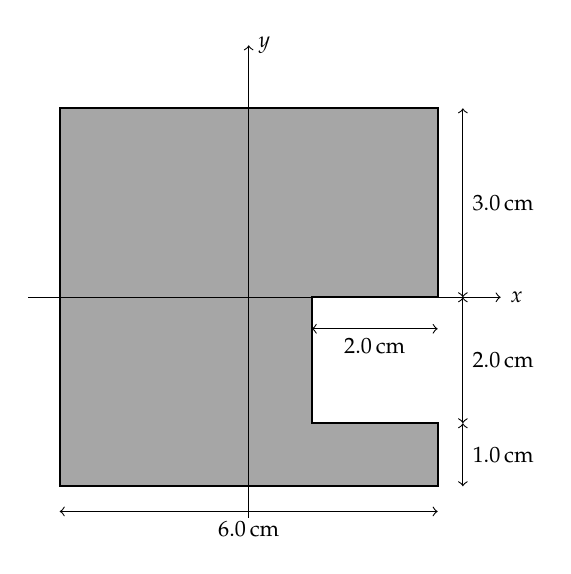
\begin{tikzpicture}[scale=0.8]
    \draw[fill=gray!70,thick](-3,-3)--(-3,3)--(3,3)--(3,0)--(1,0)--(1,-2)
    --(3,-2)--(3,-3)--cycle;
    \draw[->](-3.5,0)--(4,0) node[pos=1,right]{\footnotesize $x$};
    \draw[->](0,-3.5)--(0,4) node[pos=1,right]{\footnotesize $y$};
    \draw[<->](-3,-3.4)--(3,-3.4)
    node[midway,below]{\footnotesize\SI{6.0}{cm}};
    \draw[<->](3.4,3)--(3.4,0) node[midway,right]{\footnotesize\SI{3.0}{cm}};
    \draw[<->](3.4,0)--(3.4,-2) node[midway,right]{\footnotesize\SI{2.0}{cm}};
    \draw[<->](3.4,-2)--(3.4,-3) node[midway,right]{\footnotesize\SI{1.0}{cm}};
    \draw[<->](1,-0.5)--(3,-0.5) node[midway,below]{\footnotesize\SI{2.0}{cm}};
  \end{tikzpicture}
  \vspace{2in}  

\item Three masses are located at the locations shown below. Where should a
  \SI{5.0}{\kg} mass is to be placed such that the center of mass is at the
  origin?\\
  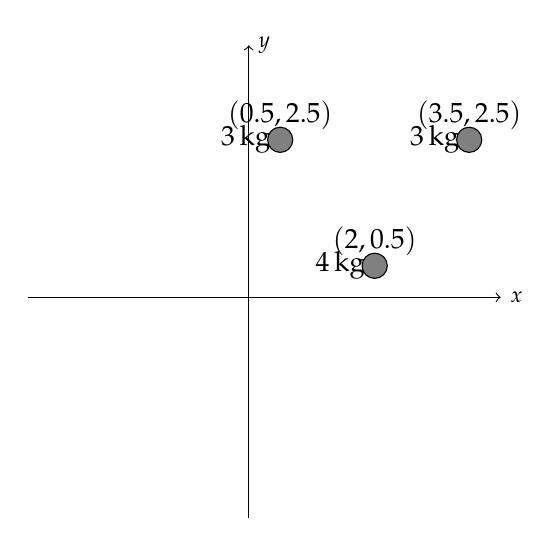
\begin{tikzpicture}[scale=0.8]
    \draw[->](-3.5,0)--(4,0) node[pos=1,right]{\footnotesize $x$};
    \draw[->](0,-3.5)--(0,4) node[pos=1,right]{\footnotesize $y$};
    \draw[fill=gray](2,0.5) circle(0.2)
    node[left]{\SI{4}{\kg}}
    node[above]{$(2,0.5)$};
    \draw[fill=gray](0.5,2.5) circle(0.2)
    node[left]{\SI{3}{\kg}}
    node[above]{$(0.5,2.5)$};
    \draw[fill=gray](3.5,2.5) circle(0.2)
    node[left]{\SI{3}{\kg}}
    node[above]{$(3.5,2.5)$};
  \end{tikzpicture}
\end{enumerate}
\end{document}
